\documentclass[12pt, fleqn]{article}
\usepackage{amsmath}
\usepackage{geometry, titling, enumitem, graphicx, float, listings, xcolor}

\graphicspath{{./images/}}

\geometry{
    paper=a4paper,
    top=64pt,
    bottom=64pt
}

\definecolor{bg}{rgb}{0.96,0.96,0.96}
\definecolor{codegray}{rgb}{0.5,0.5,0.5}
\definecolor{codepurple}{rgb}{0.58,0,0.82}
\definecolor{backcolour}{rgb}{0.95,0.95,0.92}

\lstset{
    basicstyle=\ttfamily\small,
    backgroundcolor=\color{gray!5},
    frame=single,
    rulecolor=\color{gray!20},
    framesep=16pt,
    xleftmargin=16pt,
    xrightmargin=16pt,
    captionpos=b
}

\renewcommand{\arraystretch}{1.2}
\setlength{\tabcolsep}{8pt}

\NewDocumentCommand{\course}{m}{\gdef\thecourse{#1}}
\NewDocumentCommand{\authors}{m}{\gdef\theauthors{#1}}
\NewDocumentCommand{\professor}{m}{\gdef\theprofessor{#1}}
\NewDocumentCommand{\semester}{m}{\gdef\thesemester{#1}}

\renewcommand{\maketitle}{
    \begin{titlepage}
        \begin{center}
            {\scshape Universidade Federal do Rio Grande do Sul\\Instituto de Informática} \\
            \vspace*{\fill}
            {\large \thecourse} \\[16pt]
            {\Huge \thetitle} \\[36pt]
            \theauthors \\
            \vspace*{\fill}
            \theprofessor \\[2pt]
            \thesemester
        \end{center}
    \end{titlepage}
}

\course{Circuitos Digitais – INF01058}
\title{LAB 05 – ULA}
\authors{
    Ana Cláudia Rodrigues — 343123 \\[2pt]
    Bruno Samuel Ardenghi Gonçalves — 550452
}
\professor{Prof. Sérgio Bampi}
\semester{2025/1}

\begin{document}

\maketitle

\section{Introdução}

Neste laboratório desenvolvemos uma versão de Unidade Lógica e Aritmética (ULA), a qual possui operação artmética de soma e operações lógicas de AND, OR e NOT. O projeto foi implementado e simulado pelo software Quartus, posteriormente sintetizado e testado em uma FPGA Cyclone III D0 (modelo EP3C16F484C6).

\subsection{Entradas}

\begin{itemize}
    \item $A_{3-0}$: primeiro operando
    \item $B_{3-0}:$ segundo operando
    \item $op\_sel_{1-0}$: seletor de operação
\end{itemize}

\subsection{Saídas}

\begin{itemize}
    \item $S_{3-0}$: resultado da operação
    \item $flag\_Z$: indicador de resultado igual a zero ($S_n = 0$)
    \item $flag\_N$: indicador de resultado negativo ($S_3 = 1$)
\end{itemize}

\subsection{Módulos e funções}

\begin{itemize}
    \item Mutiplexador 4:1 de 4 bits
        \begin{align*}
            S_n &= ((A_n\cdot \overline{op\_sel_n})+(B_n\cdot op\_sel_n))
        \end{align*}
        OBS: para a lógica de dois níveis implementada no circuito, temos:
        \begin{align*}
            S_n = (((\text{RCA}\cdot \overline{op\_sel_0}) + (\text{AND}\cdot op\_sel_0))\cdot\overline{op\_sel_1}) \\
            +(((\text{OR}\cdot \overline{op\_sel_0})+(\text{NOT}\cdot op\_sel_0))\cdot op\_sel_1)
        \end{align*}
    \item Ripple Carry Adder (RCA) de 4 bits
        \begin{align*}
            C_0 &= A_0 \cdot B_0 \\
            S_0 &= A_0 \oplus B_0 \\
            C_{n \ge 1} &= \overline{\overline{((A_n \oplus B_n) \cdot C_{n-1})} \cdot \overline{(A_n \cdot B_n)}} \\
            S_{n \ge 1} &= (A_n \oplus B_n) \oplus C_{n-1} \\
        \end{align*}
    \item AND de 4 bits
        \begin{align*}
            S_n = A_n \cdot B_n
        \end{align*}
    \item OR de 4 bits
        \begin{align*}
            S_n = A_n + B_n
        \end{align*}
    \item NOT de 4 bits
        \begin{align*}
            S_n = \overline{A_n}
        \end{align*}
\end{itemize}

\section{Resultados}

\begin{table}[H]
    \centering
    \begin{tabular}{|l | c|}
        \hline
        \textbf{Total de elementos lógicos} & 11 \\
        \hline
        \textbf{Total de pinos} & 16 \\
        \hline
        \textbf{Área total} & 27 \\
        \hline
    \end{tabular}
    \caption{Consumo de recursos do FPGA em área}
\end{table}

\begin{table}[H]
    \centering
    \begin{tabular}{|l | c|}
        \hline
        \textbf{Frequencia máxima} & 134.77 MHz \\
        \hline
        \textbf{Atraso crítico} & 6.920 ($B_1 \to S_2$) \\
        \hline
    \end{tabular}
    \caption{Frequência máxima de operação e atraso crítico (Slow, 85°C)}
\end{table}

\section{Capturas de tela}

\begin{figure}[H]
    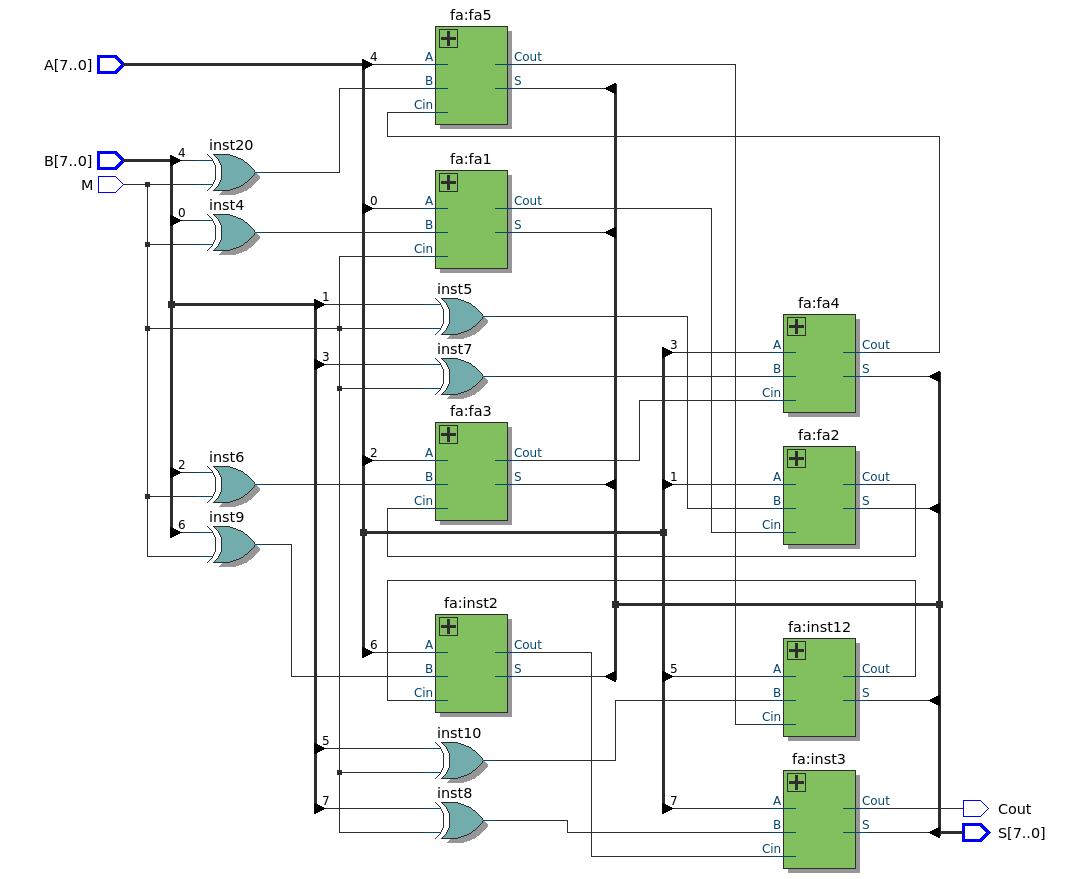
\includegraphics[width=\textwidth]{netlist.png}
    \caption{Captura de tela do netlist}
\end{figure}

\begin{figure}[H]
    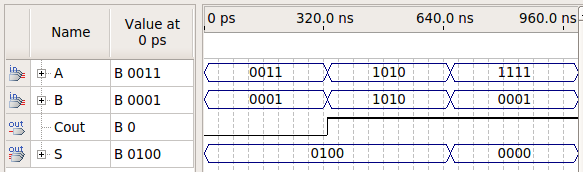
\includegraphics[width=\textwidth]{waveform.png}
    \caption{Captura de tela da simulação em forma de onda com atraso}
\end{figure}

\section{Arquivo de restrições}

\begin{lstlisting}[caption=constraints.sdc]
create_clock -name clk -period 10
set_clock_uncertainty -from clk 0.1

set_input_delay -clock clk -max 0.2 [all_inputs]
set_input_delay -clock clk -min 0.01 [all_inputs]
set_output_delay -clock clk -max 0.2 [all_outputs]
set_output_delay -clock clk -min 0.01 [all_outputs]    
\end{lstlisting}

\end{document}
